\documentclass{article}
\usepackage[utf8]{inputenc}
\usepackage{gensymb}
\usepackage{graphicx}
\usepackage{multicol}
\usepackage{amsmath}
\usepackage{amssymb}
\usepackage{physics}
\usepackage{hyperref}
\usepackage{cancel}

\graphicspath{ {./chap1images/} }

\oddsidemargin=-.3in
\evensidemargin=-.5in
\textwidth=7in
\topmargin=-1in
\textheight=10in

\parindent=.2in
\pagestyle{plain}

\title{\textbf{What is an Operation?} \\ \large Math 1 - Chapter 1}
\author{Theo Rode}
\date{}

\begin{document}

\maketitle


What do you think of when you hear the word ``operation''? It is common to think of the process of ``doing something'' as in a surgery or something similar. This is a notion that carries over to mathematics. An operation, put informally, is something which ``alters'' a number (or value) in some way. You have learned about operations before, just maybe under a different name. In fact, you are probably very familiar with two of them:
\begin{center}
    Addition and Multiplication
\end{center}

\section*{Addition}

Of course, you have all seen addition before. We can say things like: 
\[ 3 + 5 = 8\]
\[ 2 + 7 = 9 \]

The idea is that if we had the problem $3+5$, we say we are taking three of something, say we have three stones, and we add 5 stones. Together, we now have eight stones, so we say: $3+5 = 8$. We can look at this visually: 

\begin{center}
    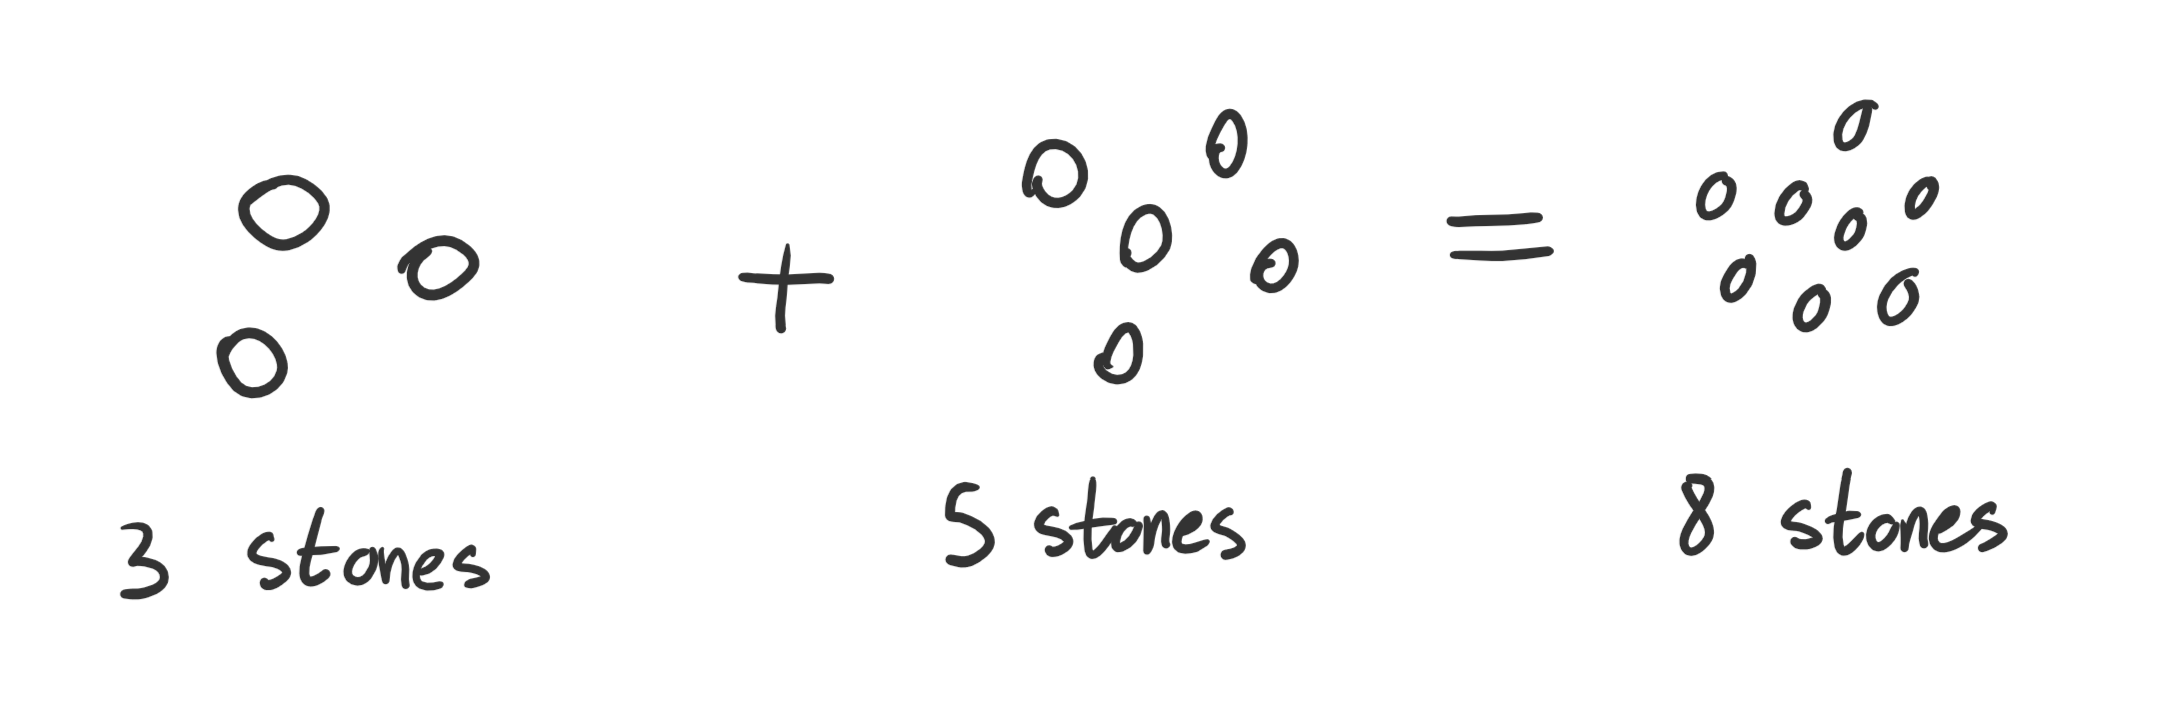
\includegraphics[scale=0.5]{chap1images/chapter1_draw1.png}
\end{center}

On both sides of the equal sign we can count 8 stones, therefore we can say that $3+5=8$. This is the physical representation of addition and its practical purpose. We needed a way to talk about the amount of ``things'' we had and it was useful to have a way to reference putting two groups of ``things'' together. 

For a very long time, we did addition by adding groups of ``stones'' together (or just groups of ``things''). You could have 1 stone, 2 stones, 3 stones, etc. Today, we call these quantities the \textit{natural numbers}. The numbers you use when you count: 
\[ 1, 2, 3, 4, \ldots \]

But using these numbers for addition leaves much to be desired. A nice quality of an operation which these numbers don't have is an \textit{identity}. What is an identity? A value we can use in an operation which doesn't change the value. In other words, the number which we can add to 5 (or really any number) such that it is still 5 (or whatever number you picked). 

Some of you might immediately know what value this is for addition, but even so, I want you to take a second to think of what number this works for. Does it exist in the natural numbers: 
\[ 1, 2, 3, 4, \ldots \]

You will find that there isn't a natural number which satisfies this. Many of you probably thought of 0, which in fact would work as the addition identity. So, needing a 0, mathematicians created the \textit{whole numbers}. These are basically the natural numbers, but with 0: 
\[ 0, 1, 2, 3, 4, \ldots \]
\newpage
You might wonder why it took a long time to consider 0 a number, but consider how it would be used in addition: 
\begin{center}
    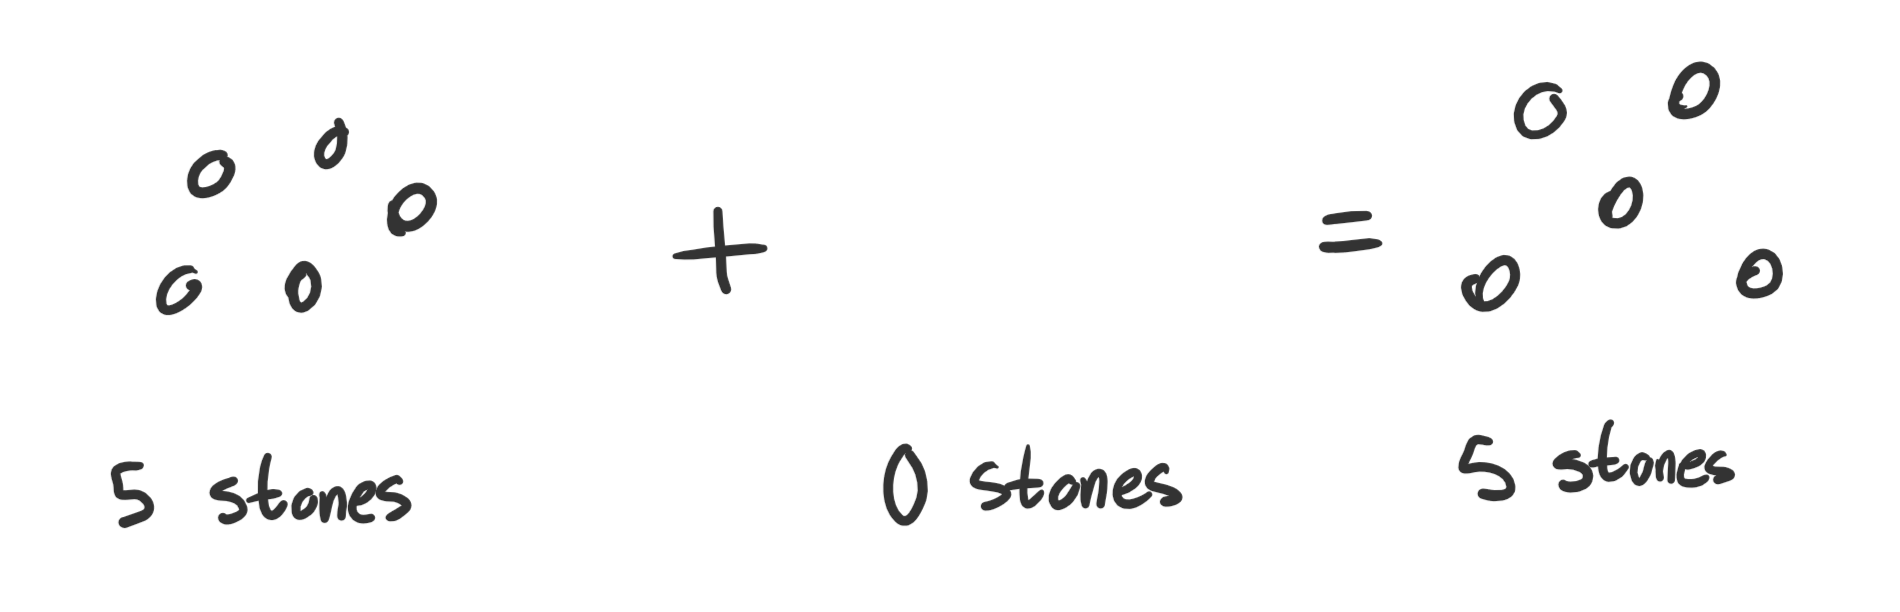
\includegraphics[scale=0.5]{chap1images/chapter1_draw2.png}
\end{center}

What does it mean to add 0 stones to 5 stones? Of course, we can think about it as adding no stones, but then what is the point of representing it as a number? Adding no stones is the same as not adding at all. I hope you at least see why this doesn't make a ton of sense in the real world. Over the next few weeks, I hope to justify to you why 0, and the identity as a concept, is useful, but for now it is just something I want you to think about. 

Getting back to the idea of the identity, we can now add 0 to any other whole number and get that whole number back: 
\[ 1 + 0 = 1 \]
\[ 2 + 0 = 2 \]
\[ 3 + 0 = 3 \]
\[ 0 + 0 = 0 \]

And note that, in the last equation, this also works for 0 itself. 0 as an identity works for any number. 

There is one more thing that would be really nice to have for an operation. A way to get back to a number. For example, if I were to add 3 to 5, I would get 8: 
\[ 5 + 3 = 8 \]

If I had 8, and I knew I had added 3 previously, how would I get back to the number I started at? How would I get back to 5? You might try a bunch of numbers before 8 until you found the answer: 
\[ 2 + 3 = 5 \text{ :(} \]
\[ 3 + 3 = 6 \text{ :(} \]
\[ 4 + 3 = 7 \text{ :(} \]
\[ 5 + 3 = 8 \text{ !!! :)} \]

But this could be time consuming for larger numbers and just doesn't seem like a good method. So, mathematicians invented the \textit{integers}. Each natural number has its own ``negative'' counterpart in the integers: 
\[ \ldots -4, -3, -2, -1, 0, 1, 2, 3, 4, \ldots \]

The negative of a given number is the \textit{additive inverse} (the inverse for addition) of that number. So in our case, adding $-3$ to $8$ should get us back to $5$: 
\[ 8 + -3 = 5 \]

What were we actually doing when we said $8 + -3 = 5$. If you really think about what we are doing here, it really doesn't make any sense. What does it mean to have -3 stones? 
\begin{center}
    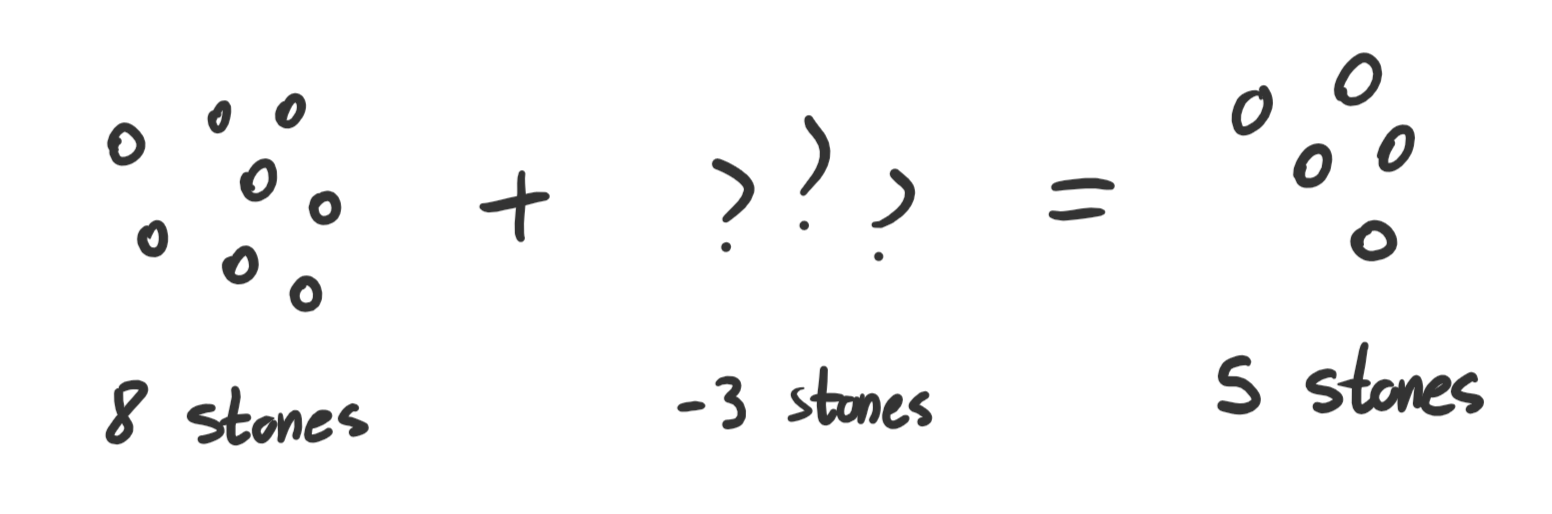
\includegraphics[scale=0.5]{chap1images/chapter1_draw3.png}
\end{center}

We can instead think about the inverse of a number as sending it to the identity. Like so: 
\[ 3 + -3 = 0 \]
\[ 4 + -4 = 0 \]
\[ 10 + -10 = 0 \]

Therefore, we could instead think about $8 + -3$ as first looking at 8 as $5+3$. We then have: $5 + 3 + -3$ and we can say that $3 + -3 = 0$. Therefore, we are left with: 
\[ 5 + 0 = 5 \]

So that you don't get confused in the future, know that \textbf{``adding by the inverse''} is typically referred to as \textbf{``subtraction.''} This is something you have probably already heard about and some of you may of thought of this when thinking about the inverse of addition. So quickly, subtraction is just adding by the inverse. We could say: 
\[ 8 + -3 = 5 \]

Or we could say: 
\[ 8 - 3 = 5 \]

This might at first seem like a better operation, but I would like you to instead think only in addition (you add by the inverse, do not use subtraction). I hope that the reasons for this become clear soon, but for know you will have to take my word for it that addition is better.

And that is addition! At least for now, there are a few other things that we still need to talk about for addition, but I hope this is a slightly new way of looking at something which you should already be fairly familiar with. 

\section*{Multiplication}

I now want to introduce you our second operation, multiplication! We can think of multiplication as ``super addition.'' What does that mean? Well lets say we have the problem: 
\[ 3 \times 5 \]

The way we would solve this is by adding 3 together 5 times: 
\[ 3 + 3 + 3 + 3 + 3 = 15 \]

In other words (or pictures), you can think about multiplication as, in the example of $3 \times 5$, adding together five groups of three: 

\begin{center}
    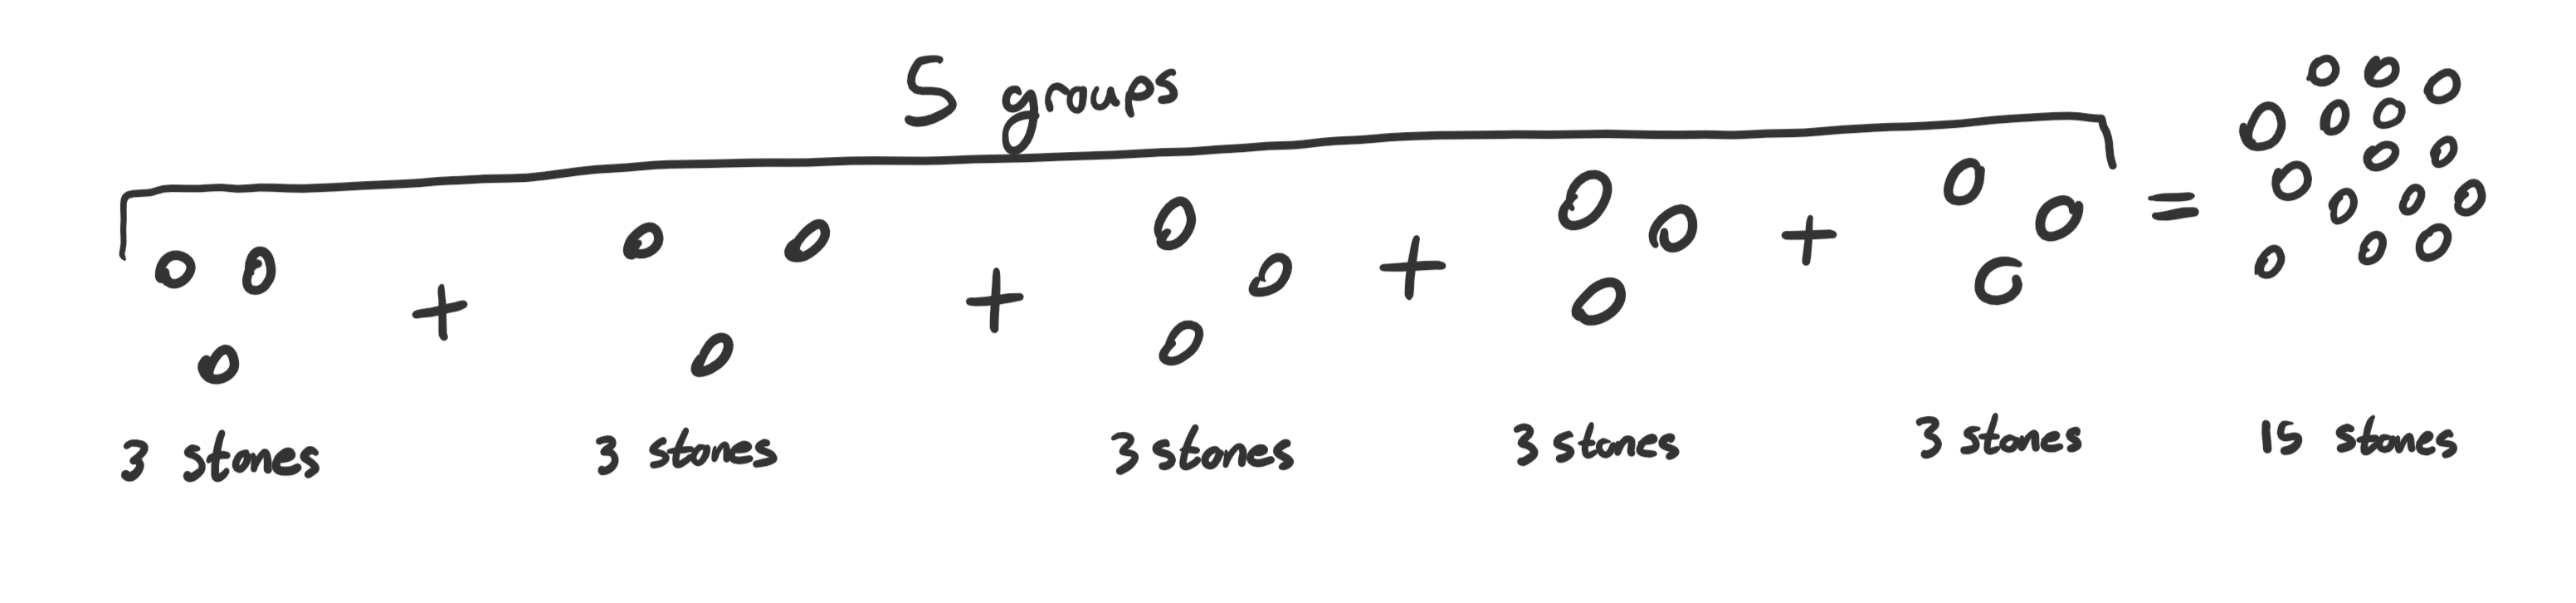
\includegraphics[scale=0.35]{chap1images/chapter1_draw4.png}
\end{center}

Now much like addition, let's think about what the \textit{identity} is for multiplication. If we remember back to addition, the identity is the number which if we multiply the identity by another number, it is still that number. 

I want you to think for a minute what this number would be? More specifically if I had the number 5 and I multiplied it by another number, which number would give the result of 5?

After a little bit of thinking, you may realize that 1 is this number. We can see: 
\[ 5 \times 1 = 5 \]
\[ 6 \times 1 = 6 \]
\[ 11 \times 1 = 11 \]

So how do we visualize multiplying by 1? Well, we looked at $3 \times 5$ as adding together 5 groups of 3. So, if we have $5 \times 1$ we can think of it as adding together 1 group of 5. What is 1 group of 5? Just 5!

\begin{center}
    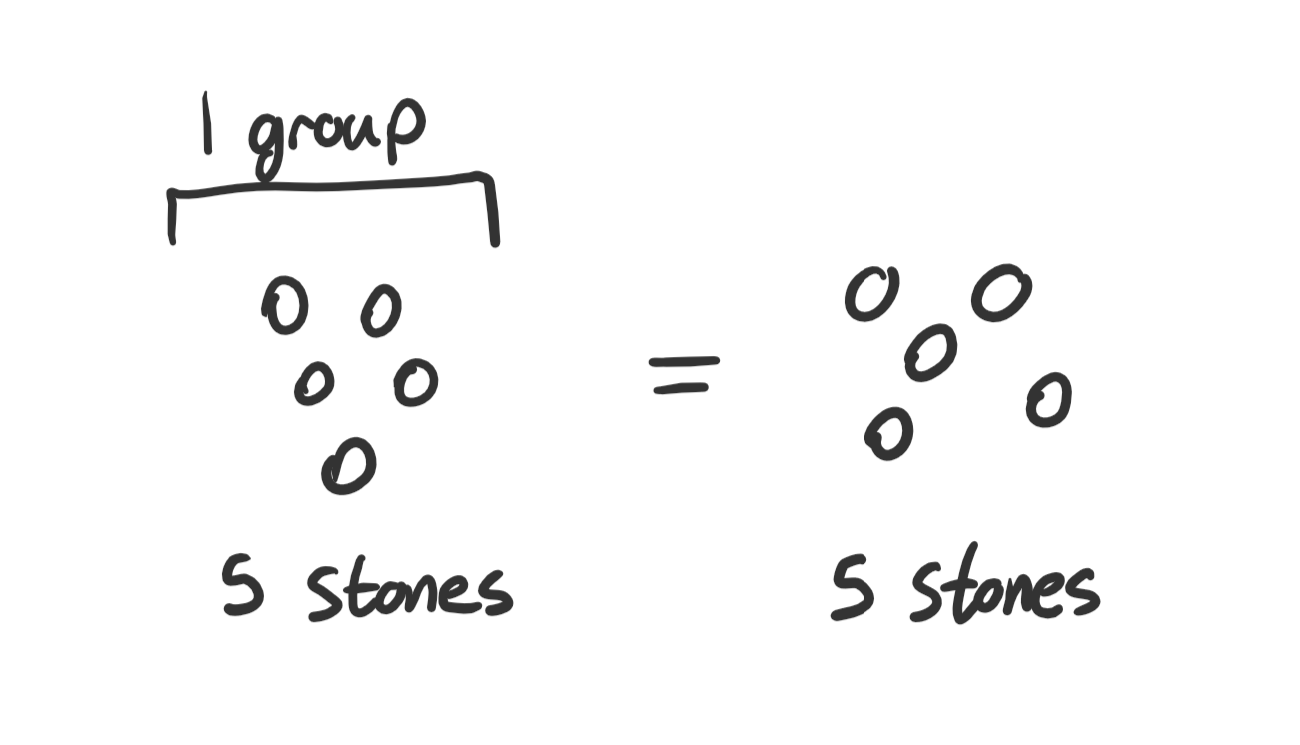
\includegraphics[scale=0.5]{chap1images/chapter1_draw5.png}
\end{center}

That's cool! Our \textit{identity} for multiplication is 1! But what about the \textit{inverse}? We defined the inverse of addition to be the negative of a number. So the inverse of adding three is adding negative three: 
\[ 5 + 3 = 8 \]
\[ 8 + -3 = 5 \]

Or we could say:
\[ 3 + -3 = 0 \]

As we know that adding the inverse of a number to itself gives us the identity. So, what would this be for multiplication? What could we multiply by to ``undo'' multiplying by 5? Multiplying by 6? In other words, what can we multiply 5 by to get the multiplicative identity, 1? 

\section*{Homework}

For homework I don't want you to do much more than think about the last question I proposed: 
\begin{center}
    What is the multiplicative inverse? 
\end{center}

If you are not super confident with addition and multiplication you can try some of the following problems, but you are by no means required to. 

\section*{Problems}
\begin{multicols*}{2}
    For the following problems, simply compute the answer:
    \begin{enumerate}
        \item $5 + 3$
        \item $2 + 4$ 
        \item $19 + 12$ 
        \item $5 + -3$
        \item $8 + -6$
        \item $12 + -14$ 
        \item $12 + -12$
        \item $7 + 0$
        \item $4 + 0$
        \item $4 \times 3$
        \item $6 \times 7$
        \item $12 \times 3$
        \item $16 \times 4$
        \item $3 \times 8$
        \item $9 \times 2$
        \item $5 \times 1$
        \item $7 \times 1$
    \end{enumerate}

    For the remaining problems, write down some thoughts and if you have an answer you can show how you got it:
    \begin{enumerate}
        \item[18. ] Why is $5 + 3$ the same as $3 + 5$? Is this true for all addition? Can we always reverse the terms and get the same result?
        \item[19. ] Is $5 \times 3$ the same as $3 \times 5$? Is this true for all multiplication? Can we always reverse the terms and get the same result?
        \item[20. ] What is the additive inverse of $0$? Why? Can you justify why this makes sense?   
    \end{enumerate}

\end{multicols*}

\end{document}
